\documentclass[11pt]{article}

\usepackage[a4paper,margin=1in]{geometry}
\usepackage[T1]{fontenc}
\usepackage[utf8]{inputenc}
\usepackage{lmodern}
\usepackage{microtype}
\usepackage{amsmath,amssymb,amsthm,mathtools}
\usepackage{booktabs}
\usepackage{array}
\usepackage{graphicx}
\usepackage{float}
\usepackage{placeins}
\usepackage{enumitem}
\usepackage[numbers,sort&compress]{natbib}
\usepackage{xcolor}
\usepackage{xurl}
\usepackage[colorlinks=true,linkcolor=blue!55!black,citecolor=blue!55!black,urlcolor=blue!55!black]{hyperref}
\usepackage[nameinlink,noabbrev]{cleveref}

\setlength{\parindent}{1.4em}
\setlength{\parskip}{0.15em}
\setlist{itemsep=0.25em,topsep=0.35em}
\allowdisplaybreaks

\newtheorem{theorem}{Theorem}[section]
\newtheorem{proposition}[theorem]{Proposition}
\newtheorem{lemma}[theorem]{Lemma}
\newtheorem{corollary}[theorem]{Corollary}
\theoremstyle{definition}
\newtheorem{definition}[theorem]{Definition}
\theoremstyle{remark}
\newtheorem{remark}[theorem]{Remark}

\newcommand{\C}{\mathbb C}
\newcommand{\Id}{\mathrm I}
\newcommand{\norm}[1]{\left\lVert#1\right\rVert}
\newcommand{\absentry}[1]{\left|#1\right|}
\newcommand{\down}{\operatorname{down}}
\newcommand{\up}{\operatorname{up}}
\newcommand{\Atilde}{\widetilde A}

\hypersetup{
  pdftitle={One-Channel Grushin Deflation of a Nonnormal Complement Resolvent},
  pdfauthor={Liang Wang},
  pdfsubject={Exact lifted-inverse budgets and a certified accretivity obstruction},
  pdfkeywords={Grushin problem, resolvent, singular deflation, interval arithmetic, numerical range}
}

\title{\textbf{One-Channel Grushin Deflation of a Nonnormal Complement Resolvent}\\[0.35em]
\large Exact Lifted-Inverse Budgets at a Quadratic Band-Merging Map\\
and a Certified Accretivity Obstruction}
\author{Liang Wang\\
\small School of Artificial Intelligence and Automation,\\[-0.2em]
\small Huazhong University of Science and Technology, Wuhan 430074, P.R. China\\
\small \texttt{wangliang.f@gmail.com}}
\date{July 2026}

\begin{document}
\maketitle

\begin{abstract}
An arcwise primal--dual Feshbach enclosure for a stored finite noisy transfer
matrix reduced its remaining matrix Rouché condition to an upper bound for
the nonnormal complement resolvent $(z\Id-B)^{-1}$.  Direct global
smallest-singular-value calculations are expensive and, without validation,
provide only lower estimates for the inverse norm.  This paper isolates the
observed near-singularity before asking for a global certificate.

For $A=z_0\Id-B$, unit directions obtained by exact normalization of stored
vectors $u,v$, a positive scalar
$\widehat s$, and residuals
\[
 r=Av-\widehat s u,\qquad q=A^*u-\widehat s v,
\]
we introduce the one-channel lift
$\widetilde A=A+(\tau-\widehat s)uv^*$.  An exact
Sherman--Morrison/Grushin calculation proves that any validated bound
$K\geq\|\widetilde A^{-1}\|_2$ implies
\[
 \|A^{-1}\|_2\leq
 K+\frac{|\tau-\widehat s|(1+K\|r\|_2)(1+K\|q\|_2)}
 {\tau(\widehat s-|\tau-\widehat s|K\|r\|_2)}.
\]
The formula yields a downward conditional budget $K_*^-$ for the lifted
inverse and combines with a center-to-arc Neumann bound.

At the budget-tightest RH-28 arc of each of seven stored scales, dimensions
range from 2048 to 204800.  Componentwise stored-factor arithmetic and
Arb-backed exact normalization enclose the right and left residuals by at
most $4.38\times10^{-10}$ and $3.56\times10^{-9}$.  Floating inverse
iteration gives arc inverse candidates from $4.57\times10^2$ to
$1.76\times10^4$.  After one-channel lifting, the candidate bulk singular
value is 11.1--34.1 times larger than the dangerous value.  The conditional
lifted-inverse budgets exceed the corresponding floating candidates by
factors from 95.0 to $1.73\times10^3$; the finest budget is
$6.29\times10^4$ versus a candidate $6.62\times10^2$.

A separate outward-rounded three-vector witness proves that the origin lies
in the compressed numerical range of the coarse lifted operator.  Hence no
rotation can make its Hermitian part positive definite: simple accretivity
cannot supply the missing bulk bound even after rank-one lifting.

The algebra, stored residuals, conditional budgets, and numerical-range
witness are rigorous for the stated stored finite model.  No upper bound for
$\|\widetilde A^{-1}\|_2$ is proved, so neither the original complement
resolvent, a full-contour Rouché transfer, a root count, a continuum limit,
nor any statement about the Riemann hypothesis is claimed.
\end{abstract}

\noindent\textbf{Keywords:} Grushin problem; nonnormal resolvent; singular
deflation; Sherman--Morrison formula; componentwise enclosure; numerical
range; interval arithmetic.

\medskip
\noindent\textbf{MSC 2020:} 47A10; 47A55; 47B65; 65F10; 65F15; 65F35;
65G20; 65P30.


\section{Introduction}
\label{sec:introduction}

The packet--complement program considered here studies finite noisy transfer
matrices near a quadratic band-merging regime.  A packet Feshbach reduction
has rank between four and nine, while its ambient complement reaches
dimension 204800.  The preceding layers constructed a holomorphic shifted
Arnoldi model, derived directional and primal--dual residual identities,
replaced ordinary residuals by outward-rounded stored-factor enclosures, and
extended those enclosures from contour nodes to an exact adaptive cover of a
mathematical circle
\citep{WangContourFeshbach2026,WangDirectionalRouche2026,WangPrimalDual2026,WangOutwardCode2026,WangArcwise2026}.

The last step isolated a sharp but difficult condition.  On every accepted
arc $a$, the exact stored finite Feshbach map $F$ and its stored rational
model $\widehat F_J$ satisfy a conditional estimate
\begin{equation}
 \norm{\widehat F_J(z)^{-1}(F(z)-\widehat F_J(z))}_2
 \leq \bar\eta_a+M\bar c_a,
 \qquad z\in a,
 \label{eq:rh28-gate}
\end{equation}
where $M$ must be an externally validated upper bound for
$\|(z\Id-B)^{-1}\|_2$.  The archived threshold
$M_{*,a}^-=(1-\bar\eta_a)/\bar c_a$ is admissible but is not an inverse
estimate.  At the finest stored scale its minimum is only
$1.10\times10^5$.

There are two reasons not to attack this condition with an unstructured
smallest-singular-value calculation.  First, a computed singular value and
small residual do not exclude an unseen smaller singular value.  Second,
the complement is strongly nonnormal: a global norm can be governed by a
very small number of directions, while the rest of the space is much better
conditioned \citep{TrefethenEmbree2005,StewartSun1990}.  A useful next step
should separate those two effects.

The present paper makes that separation with one rank-one lift.  The main
contributions are:
\begin{enumerate}
 \item an exact one-channel inverse bound that converts a certificate for a
       lifted, better-conditioned operator into a certificate for the
       original complement shift;
 \item a downward conditional budget for the lifted inverse, including
       exact center-to-arc transport;
 \item a seven-scale audit at the budget-tightest RH-28 arc, with
       componentwise stored-factor residuals and Arb-backed exact
       normalization;
 \item a certified numerical-range obstruction showing that rank-one
       lifting does not make a simple accretivity proof available.
\end{enumerate}

The outcome is a genuine reduction, not a closure theorem.  At the finest
selected arc, the original floating margin over the RH-28 threshold is only
6.24.  The one-channel reduction asks instead for a bound
$\|\Atilde^{-1}\|_2<6.29\times10^4$, while its floating candidate is
$6.62\times10^2$.  This roughly 95-fold separation identifies a much more
forgiving target for a validated sparse or block-Grushin inverse method.

\subsection{Evidence hierarchy}

Three levels are kept separate throughout.
\begin{enumerate}
 \item \emph{Exact stored-model statements}: the rank-one identities,
       inverse inequalities, normalization bounds, componentwise residual
       enclosures, downward budgets, and the numerical-range witness.
 \item \emph{Conditional statements}: if a validated upper bound for the
       lifted inverse lies below the tabulated $K_*^-$, then the original
       center inverse and its selected RH-28 arc satisfy the required bound.
 \item \emph{Floating evidence}: inverse-iteration singular values,
       candidate inverse norms, gap ratios, and GMRES iteration counts.
\end{enumerate}
No floating candidate is used as an upper bound in a theorem.


\section{The selected complement shifts}
\label{sec:model}

For the stored packet/complement decomposition, let
\begin{equation}
 B=QU^2Q,\qquad Q=\Id-VW,
 \label{eq:complement-block}
\end{equation}
where $U$ is the stored Perron/parity-extracted one-step factor and $WV=\Id$
on the packet space.  The ambient shifted complement is
\begin{equation}
 A(z)=z\Id-B.
 \label{eq:shifted-complement}
\end{equation}
All matrices are finite.  The sparse transfer factor, peripheral modes,
packet maps, and spectral parameters are the stored binary64 values used by
RH-24--RH-28.

For each noise scale, RH-28 archived an exact dyadic circle partition.  We
select the arc with the smallest $M_{*,a}^-$, write its disc center and radius
as $z_0$ and $\rho$, and abbreviate
\[
 A=A(z_0).
\]
This is the tightest \emph{budget} arc.  It need not be the point of largest
resolvent on the full contour; the experiment therefore does not replace a
full-contour audit.

\begin{lemma}[Center-to-arc transport]
\label{lem:arc-transport}
Suppose $A(z_0)$ is invertible and
$\|A(z_0)^{-1}\|_2\leq M_0$ with $\rho M_0<1$.  Then for every
$|z-z_0|\leq\rho$,
\begin{equation}
 \norm{A(z)^{-1}}_2
 \leq \frac{M_0}{1-\rho M_0}.
 \label{eq:arc-neumann}
\end{equation}
\end{lemma}

\begin{proof}
Since $A(z)=A(z_0)+(z-z_0)\Id$, factor
\[
 A(z)=A(z_0)\bigl(\Id+(z-z_0)A(z_0)^{-1}\bigr)
\]
and apply the Neumann lemma.
\end{proof}

If $L_a$ is the downward RH-28 threshold and $\rho_a$ is an upper arc-disc
radius, it is sufficient to prove the center bound
\begin{equation}
 \norm{A(z_0)^{-1}}_2<T_a^-:=
 \down\frac{L_a}{1+\rho_aL_a}.
 \label{eq:center-budget}
\end{equation}
The implementation evaluates the denominator upward and the quotient
downward.


\section{One-channel Grushin lift}
\label{sec:grushin}

Let $u,v\in\C^n$ be unit vectors, let $\widehat s>0$, and define the two
stored-direction residuals
\begin{equation}
 r=Av-\widehat s u,
 \qquad
 q=A^*u-\widehat s v.
 \label{eq:singular-residuals}
\end{equation}
The vectors need not be exact singular vectors.  Choose a lift
$\tau>0$ and put
\begin{equation}
 c=\tau-\widehat s,
 \qquad
 \Atilde=A+cuv^*.
 \label{eq:lifted-operator}
\end{equation}
Then
\begin{equation}
 \Atilde v=\tau u+r,
 \qquad
 \Atilde^*u=\tau v+q.
 \label{eq:lifted-residuals}
\end{equation}
For an exact singular pair, the lift replaces the singular value
$\widehat s$ by $\tau$ and leaves the other singular directions unchanged.
For an approximate pair, \cref{eq:lifted-residuals} quantifies the failure of
that ideal block separation.

\begin{theorem}[One-channel lifted-inverse bound]
\label{thm:lifted-bound}
Assume $\Atilde$ is invertible and
\begin{equation}
 \norm{\Atilde^{-1}}_2\leq K.
 \label{eq:bulk-bound}
\end{equation}
If
\begin{equation}
 \delta_K:=\widehat s-|c|K\norm{r}_2>0,
 \label{eq:delta-k}
\end{equation}
then $A$ is invertible and
\begin{equation}
 \boxed{
 \norm{A^{-1}}_2
 \leq \Phi(K):=
 K+\frac{|c|(1+K\norm{r}_2)(1+K\norm{q}_2)}
 {\tau(\widehat s-|c|K\norm{r}_2)}.}
 \label{eq:phi-k}
\end{equation}
\end{theorem}

\begin{proof}
The first identity in \cref{eq:lifted-residuals} gives
\begin{equation}
 \Atilde^{-1}u=\frac{1}{\tau}
 \bigl(v-\Atilde^{-1}r\bigr),
 \qquad
 \norm{\Atilde^{-1}u}_2\leq\frac{1+K\norm r_2}{\tau}.
 \label{eq:right-lifted-solve}
\end{equation}
The adjoint identity similarly gives
\begin{equation}
 \Atilde^{-*}v=\frac{1}{\tau}
 \bigl(u-\Atilde^{-*}q\bigr),
 \qquad
 \norm{\Atilde^{-*}v}_2\leq\frac{1+K\norm q_2}{\tau}.
 \label{eq:left-lifted-solve}
\end{equation}
Since $A=\Atilde-cuv^*$, the Sherman--Morrison denominator is
\[
 d=1-cv^*\Atilde^{-1}u.
\]
Using \cref{eq:right-lifted-solve} before taking norms,
\[
 d=\frac{\widehat s}{\tau}
   +\frac{c}{\tau}v^*\Atilde^{-1}r,
 \qquad
 |d|\geq\frac{\widehat s-|c|K\norm r_2}{\tau}
 =\frac{\delta_K}{\tau}>0.
\]
Thus the rank-one inverse formula is valid:
\[
 A^{-1}=\Atilde^{-1}
 +\frac{c}{d}\Atilde^{-1}u v^*\Atilde^{-1}.
\]
Insert the two solve bounds and the lower bound for $|d|$ to obtain
\cref{eq:phi-k} \citep{ShermanMorrison1950,SjoestrandZworski2007}.
\end{proof}

\begin{remark}
The theorem does not assume that $\widehat s$ is the smallest singular value.
It is therefore legitimate to treat the computed binary64 vectors and scalar
as exact stored inputs.  Their quality enters only through $\|r\|$ and
$\|q\|$.
\end{remark}

For fixed nonnegative residual bounds, $\Phi(K)$ is increasing on the
admissible interval $\delta_K>0$.  This produces the next conditional gate.

\begin{corollary}[Lifted bulk budget]
\label{cor:bulk-budget}
Let $T_a^-$ be the center budget in \cref{eq:center-budget}.  Define
\begin{equation}
 K_{*,a}^-=down\sup\{K\geq0:
 \delta_K>0,\ \Phi(K)<T_a^-\}.
 \label{eq:bulk-budget}
\end{equation}
If a validated bound satisfies
$\|\Atilde^{-1}\|_2<K_{*,a}^-$, then the original inverse satisfies the
RH-28 requirement throughout the selected arc.
\end{corollary}

The code computes \cref{eq:bulk-budget} by monotone bisection with every
scalar majorant rounded upward and the final budget rounded downward.  In
the experiments $\tau=1$.


\section{Exact normalization of stored directions}
\label{sec:normalization}

Inverse iteration produces stored vectors $u_0,v_0$ whose floating norms are
close to one but not exactly one as real numbers.  Let
\[
 \alpha=\norm{u_0}_2,
 \qquad
 \beta=\norm{v_0}_2,
 \qquad
 u=u_0/\alpha,
 \qquad
 v=v_0/\beta.
\]
The exact norms of the binary64 vectors are enclosed by 160-bit Arb sums of
squares.  No floating normalization is silently promoted to an exact unit
identity.

Suppose the raw stored equations have outward residual bounds
\begin{equation}
 \norm{Av_0-\widehat s u_0}_2\leq R_0,
 \qquad
 \norm{A^*u_0-\widehat s v_0}_2\leq Q_0.
 \label{eq:raw-residuals}
\end{equation}

\begin{proposition}[Normalization transfer]
\label{prop:normalization}
For the exact unit vectors $u,v$ above,
\begin{align}
 \norm{Av-\widehat s u}_2
 &\leq \frac{R_0+\widehat s|\alpha-\beta|}{\beta},
 \label{eq:normalized-right}\\
 \norm{A^*u-\widehat s v}_2
 &\leq \frac{Q_0+\widehat s|\alpha-\beta|}{\alpha}.
 \label{eq:normalized-left}
\end{align}
\end{proposition}

\begin{proof}
For the first equation,
\[
 Av-\widehat s u
 =\frac{Av_0-\widehat s u_0}{\beta}
 +\widehat s u_0\left(\frac1\beta-\frac1\alpha\right).
\]
Since $\|u_0\|_2=\alpha$, the second term has norm
$\widehat s|\alpha-\beta|/\beta$.  The adjoint equation is identical with
$\alpha$ and $\beta$ interchanged.
\end{proof}

The raw residuals in \cref{eq:raw-residuals} are evaluated by the complete
componentwise graph inherited from RH-27.  The graph includes sparse transfer
actions, peripheral subtraction, packet projection, adjoint actions, and
spectral shifts.  Each stored binary64 factor is treated as exact input;
round-to-nearest operation centers are accompanied by outward componentwise
radii using conservative $\gamma_k$ factors
\citep{Higham2002,Rump2010,MooreKearfottCloud2009}.


\section{Floating reconnaissance and seven-scale audit}
\label{sec:numerics}

\subsection{Inverse normal iteration}

At each selected center, a deterministic starting vector is repeatedly
mapped by
\begin{equation}
 v_{j+1}\propto A^{-1}A^{-*}v_j.
 \label{eq:inverse-iteration}
\end{equation}
The two inverse actions are computed by unrestarted outer inverse iteration
and restarted GMRES inner solves.  This is a reconnaissance tool, not a
validated inverse.  At the coarse scale, one-channel inverse iteration
reproduces a PROPACK candidate to displayed precision while reducing the
wall time from about 130 seconds to 1.3 seconds.

The final stored direction is used to define $u_0=Av_0/\|Av_0\|_2$ and
$\widehat s=\|Av_0\|_2$ in binary64.  The stored-factor graph then reevaluates
both residuals independently of the inner GMRES stopping tests.  Triplet
vectors, source hashes, result hashes, and software versions are archived.

\subsection{Original tightest-arc gate}

\Cref{tab:original-gate} reports the floating center singular candidate,
its Neumann transport over the selected RH-28 arc, the archived RH-28
threshold, and their ratio.  These ratios are diagnostics only.

\begin{table}[H]
\centering
\small
\setlength{\tabcolsep}{5pt}
\caption{Floating diagnostics at the budget-tightest RH-28 arc.  The fourth
column is the center candidate transported over the archived arc disc.  The
last column is a candidate margin, not a certified resolvent ratio.}
\label{tab:original-gate}
\begin{tabular}{rrrrrr}
\toprule
$\sigma$ & $n$ & $\widehat s$ & arc $M_{\rm cand}$ & $M_{*,a}^-$ & margin \\
\midrule
$10^{-2}$ & 2,048 & $2.2867\times10^{-3}$ & $4.5744\times10^2$ & $3.9726\times10^{13}$ & $8.68\times10^{10}$ \\
$4\times10^{-3}$ & 5,120 & $1.7241\times10^{-3}$ & $5.8988\times10^2$ & $5.9371\times10^{11}$ & $1.01\times10^9$ \\
$2\times10^{-3}$ & 10,240 & $1.4263\times10^{-3}$ & $7.0665\times10^2$ & $9.9689\times10^{10}$ & $1.41\times10^8$ \\
$10^{-3}$ & 20,480 & $2.3860\times10^{-4}$ & $4.2736\times10^3$ & $3.1793\times10^9$ & $7.44\times10^5$ \\
$5\times10^{-4}$ & 40,960 & $3.0450\times10^{-4}$ & $3.3493\times10^3$ & $5.0691\times10^8$ & $1.51\times10^5$ \\
$2\times10^{-4}$ & 102,400 & $1.1833\times10^{-4}$ & $8.6451\times10^3$ & $4.0368\times10^7$ & $4.67\times10^3$ \\
$10^{-4}$ & 204,800 & $5.8108\times10^{-5}$ & $1.7625\times10^4$ & $1.0999\times10^5$ & $6.24$ \\
\bottomrule
\end{tabular}
\end{table}

The finest point is informative: the observed resolvent scale lies below
the RH-28 threshold, but only by a factor 6.24.  A loose normwise validation
could easily destroy this margin.

\subsection{Deflated bulk gate}

\Cref{tab:deflated-gate} gives the exact stored-model residual majorant
$\max(\bar r,\bar q)$, the downward lifted-inverse budget $K_*^-$, a floating
candidate $K_{\rm cand}=1/s_{\rm bulk}$, their ratio, and the observed
singular separation $s_{\rm bulk}/\widehat s$.

\begin{table}[H]
\centering
\small
\setlength{\tabcolsep}{5pt}
\caption{One-channel deflation.  Residuals and $K_*^-$ are outward/downward
stored-model quantities.  The bulk inverse, margin, and gap are floating
diagnostics.}
\label{tab:deflated-gate}
\begin{tabular}{rrrrrr}
\toprule
$\sigma$ & $\max(\bar r,\bar q)$ & $K_*^-$ & $K_{\rm cand}$ & $K_*^-/K_{\rm cand}$ & gap \\
\midrule
$10^{-2}$ & $4.416\times10^{-11}$ & $9.4974\times10^3$ & $1.5930\times10^1$ & 596 & 27.45 \\
$4\times10^{-3}$ & $6.172\times10^{-11}$ & $3.4054\times10^4$ & $2.9355\times10^1$ & $1.16\times10^3$ & 19.76 \\
$2\times10^{-3}$ & $3.908\times10^{-10}$ & $8.8744\times10^4$ & $6.2931\times10^1$ & $1.41\times10^3$ & 11.14 \\
$10^{-3}$ & $2.703\times10^{-10}$ & $2.1275\times10^5$ & $1.2283\times10^2$ & $1.73\times10^3$ & 34.12 \\
$5\times10^{-4}$ & $8.014\times10^{-10}$ & $1.6525\times10^5$ & $1.5383\times10^2$ & $1.07\times10^3$ & 21.35 \\
$2\times10^{-4}$ & $2.438\times10^{-9}$ & $3.4461\times10^5$ & $3.3421\times10^2$ & $1.03\times10^3$ & 25.29 \\
$10^{-4}$ & $3.559\times10^{-9}$ & $6.2911\times10^4$ & $6.6194\times10^2$ & 95.0 & 26.00 \\
\bottomrule
\end{tabular}
\end{table}

\begin{figure}[H]
\centering
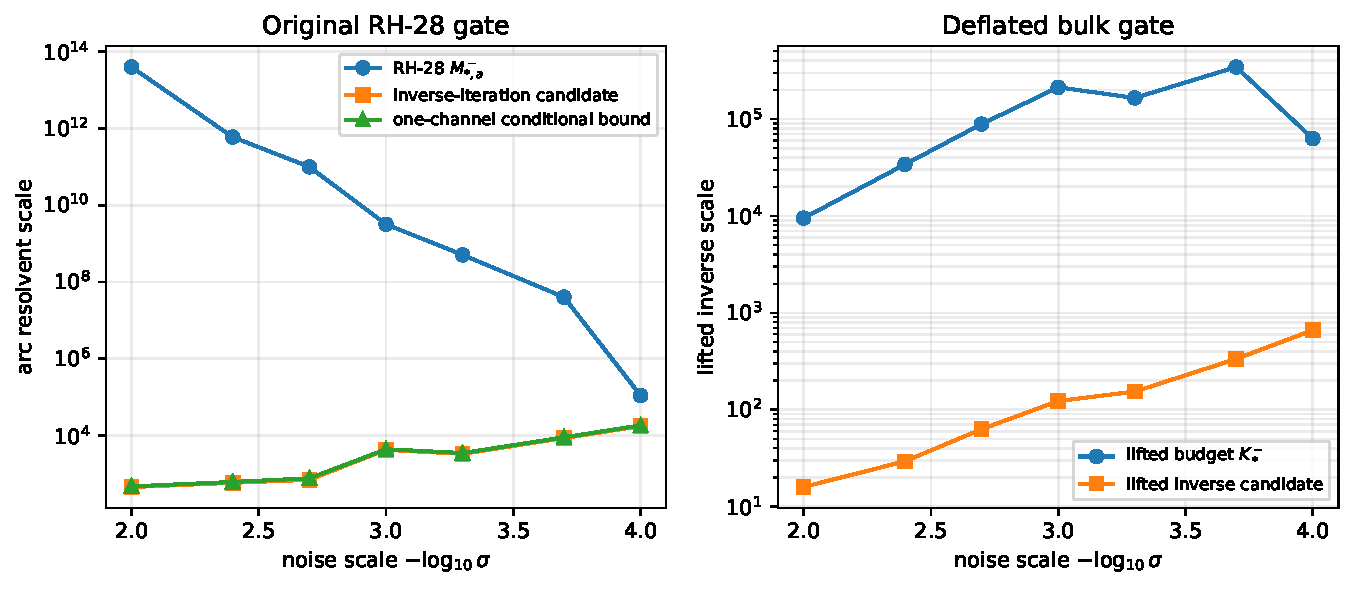
\includegraphics[width=0.98\textwidth]{figures/deflated_budget_summary.pdf}
\caption{Left: the original RH-28 arc threshold and two floating inverse
diagnostics.  Right: the exact conditional lifted-inverse budget and the
floating lifted candidate.  The large vertical separation on the right is
the practical gain from one-channel deflation.}
\label{fig:budget-summary}
\end{figure}

\begin{figure}[H]
\centering
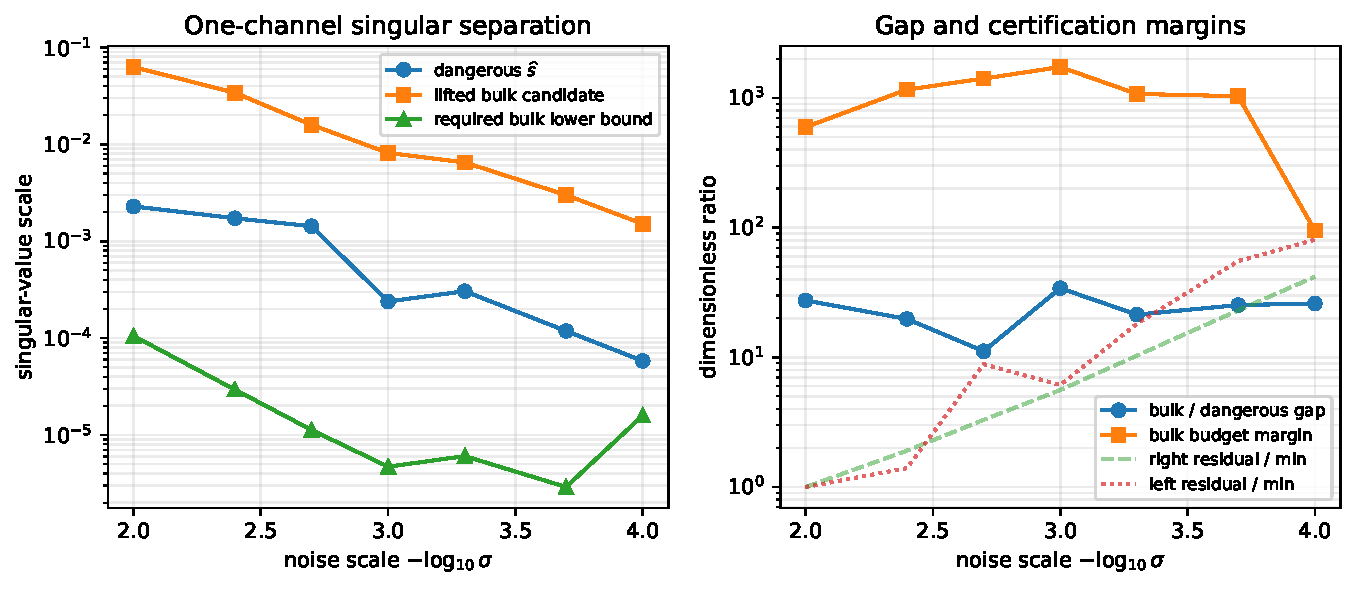
\includegraphics[width=0.98\textwidth]{figures/deflated_gap_summary.pdf}
\caption{One-channel separation.  The lifted bulk candidate exceeds the
dangerous singular candidate by factors 11.1--34.1 and lies well above the
singular lower bound $1/K_*^-$ required by the conditional theorem.}
\label{fig:gap-summary}
\end{figure}

At the finest selected arc, inserting the floating bulk candidate into the
\emph{rigorous formula} $\Phi$ gives a conditional center bound
$1.80\times10^4$ and an arc-transported value $1.84\times10^4$.  This
calculation is still floating because $K_{\rm cand}$ has not been proved to
upper-bound $\|\Atilde^{-1}\|_2$.  Its purpose is to show that the exact
formula itself does not consume the available RH-28 margin.


\section{Why accretivity still fails}
\label{sec:no-go}

A natural way to bound a resolvent is to rotate the operator until its
Hermitian part is positive.  If
\[
 \lambda_{\min}\Re(e^{-i\phi}\Atilde)\geq\gamma>0,
\]
then $\|\Atilde^{-1}\|_2\leq1/\gamma$.  The one-channel lift removes the
smallest observed singular direction, but it cannot change all numerical-
range geometry.

\begin{proposition}[Compressed numerical-range invariance]
\label{prop:numerical-range-invariance}
For every unit vector $x$ satisfying $v^*x=0$,
\begin{equation}
 x^*\Atilde x=x^*Ax.
 \label{eq:quadratic-invariance}
\end{equation}
Consequently the numerical range of $\Atilde$ contains the convex hull of
the compressed quadratic values
\[
 \{x^*Ax:\ \norm x_2=1,\ v^*x=0\}.
\]
If that convex hull contains the origin, no rotation of $\Atilde$ has a
positive-definite Hermitian part.
\end{proposition}

\begin{proof}
The rank-one term contributes
$c\,x^*uv^*x=0$, proving \cref{eq:quadratic-invariance}.  The numerical range
is convex by the Toeplitz--Hausdorff theorem \citep{HornJohnson2013}.  If a
rotation had Hermitian part bounded below by $\gamma>0$, its numerical range
would lie in the strict half-plane
$\Re(e^{-i\phi}z)\geq\gamma$, which excludes the origin.
\end{proof}

At $\sigma=10^{-2}$, three stored witness vectors were generated and then
reevaluated by the complete componentwise factor graph.  Their normalized
lifted Rayleigh values are enclosed by
\begin{align*}
 w_1&\in[-0.822329596932,-0.822329596907]
       +i[-0.448800234546,-0.448800234521],\\
 w_2&\in[0.217860304077,0.217860304097]
       +i[-1.146076361491,-1.146076361471],\\
 w_3&\in[0.011722834533,0.011722834558]
       +i[0.221374605040,0.221374605065].
\end{align*}
An Arb interval solve for barycentric weights gives
\begin{align*}
 \lambda_1&\in[0.048224961594,0.048224961982],\\
 \lambda_2&\in[0.138253914403,0.138253914615],\\
 \lambda_3&\in[0.813521123614,0.813521123792],
\end{align*}
with $\lambda_1+\lambda_2+\lambda_3=1$ and
$\lambda_1w_1+\lambda_2w_2+\lambda_3w_3=0$.  Every weight has a strictly
positive lower endpoint.  Thus the origin-in-convex-hull statement is a
stored-model certificate, not a plot-based inference.

\begin{figure}[H]
\centering
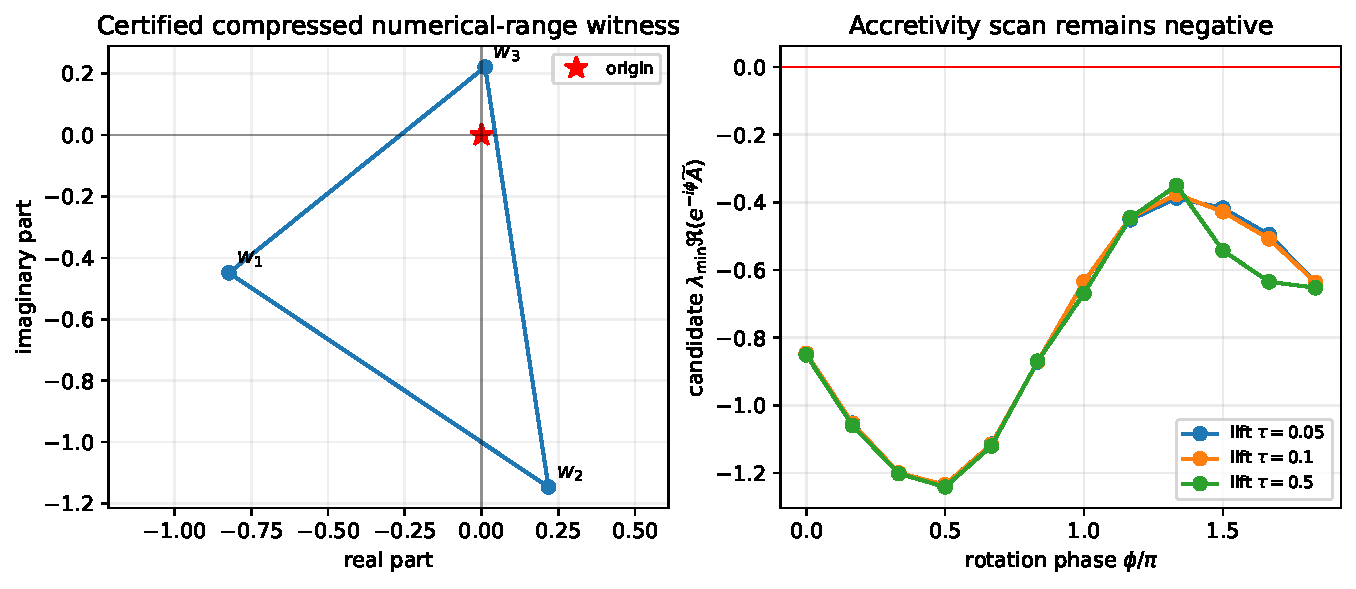
\includegraphics[width=0.98\textwidth]{figures/numerical_range_no_go.pdf}
\caption{Left: the certified three-point numerical-range witness contains
the origin.  Interval widths are much smaller than the markers.  Right:
floating phase scans for three lift values; all sampled minimum Hermitian
eigenvalues remain negative, consistent with the exact obstruction.}
\label{fig:numerical-range}
\end{figure}

This no-go result is limited but useful.  It does not rule out a validated
inverse for $\Atilde$.  It rules out obtaining that inverse merely by a
global rotated-Hermitian coercivity estimate.  A future certificate must use
more structure: a sparse approximate inverse, a further block decomposition,
or a validated normal-equation/Grushin solve.


\section{What is proved and what remains}
\label{sec:scope}

The exact stored-model achievements are:
\begin{enumerate}
 \item the one-channel residual identities and the inverse bound
       \cref{thm:lifted-bound};
 \item downward center and lifted-inverse budgets for a selected arc;
 \item componentwise stored-factor right and left residual enclosures at all
       seven budget-tightest arcs;
 \item Arb-backed exact normalization of every stored dangerous direction;
 \item a certified coarse-scale numerical-range obstruction to any global
       accretivity proof after rank-one lifting.
\end{enumerate}

The following are \emph{not} proved:
\begin{enumerate}
 \item No upper bound for $\|\Atilde^{-1}\|_2$ is supplied.  The tabulated
       $K_{\rm cand}$ values are floating candidates.
 \item Only the budget-tightest RH-28 arc at each scale is audited here.  A
       complete contour needs validated lifted bounds on a covering family
       and a certified transport of the dangerous channel.
 \item The RH-28 base winding, interior analyticity, and complement pole
       count are not validated.
 \item The stored sparse transfer matrix is not enclosed relative to an
       exact Gaussian integral operator, exact critical constants, or exact
       spectral projectors.
 \item No small-noise limit, self-adjoint generator, Hilbert--Pólya
       construction, Riemann-zero identification, or Riemann-hypothesis
       consequence is asserted.
\end{enumerate}

The main practical conclusion is quantitative.  At the finest selected arc,
the original observed resolvent has only a factor-6.24 margin over the RH-28
threshold.  After one-channel deflation, the missing validated bulk inverse
may be almost two orders of magnitude larger than its observed candidate and
still close the exact bound.  The dangerous direction is therefore worth
handling analytically rather than forcing a global norm estimator to resolve
it together with the bulk.


\section{Conclusion and next gate}
\label{sec:conclusion}

RH-28 reduced the contour comparison to a complement-resolvent upper bound.
The present paper does not manufacture that bound from floating singular
values.  Instead, it proves an exact rank-one reduction that removes the one
observed near-singular channel and replaces the original inverse gate by a
better-conditioned lifted-bulk gate.  Across seven selected arcs, the
observed singular separation is at least 11.1, and the conditional lifted
budgets exceed the corresponding candidates by at least 95.0.

The next falsifiable task is now narrower:
\begin{equation}
 \text{construct a validated upper bound for }
 \norm{\Atilde(z_0)^{-1}}_2
 \quad\text{below}\quad K_{*,a}^-,
 \label{eq:next-gate}
\end{equation}
first at the finest selected center and then on a contour covering family.
The numerical-range certificate proves that a one-line accretivity estimate
cannot do this.  Promising remaining tools are a validated sparse
approximate inverse for the lifted operator, a two-level block-Grushin
factorization, or an interval normal-equation solve that explicitly retains
the lifted channel.  Only after that gate is closed should the program return
to base winding, interior pole counting, and finite-section/continuous-model
questions.


\appendix

\section{Outward scalar conventions}
\label{app:rounding}

Every nonnegative scalar addition and multiplication in the budget code is
followed by a successor operation toward $+\infty$.  Positive denominators
are rounded toward zero before upper division; final admissible budgets are
rounded toward zero.  Vector norms are evaluated by Arb at 160 bits from the
exact binary64 real and imaginary components.  The numerical-range witness
uses 192-bit Arb interval linear algebra.  Componentwise sparse and dense
products use conservative operation-count factors under the standard
round-to-nearest model, assuming finite intermediates and no harmful
underflow.

\section{Reproduction}
\label{app:reproduction}

From this directory, the unit tests and figures are reproduced with
\begin{verbatim}
/root/math/.venv/bin/python -m pytest -q
/root/math/.venv/bin/python experiments/make_figures.py
\end{verbatim}
One stored scale is regenerated with, for example,
\begin{verbatim}
OPENBLAS_NUM_THREADS=16 /root/math/.venv/bin/python \
  experiments/run_deflated_certificate.py --sigma 0.0001
\end{verbatim}
The expensive calculations are run one physical scale per process.  The
archived triplet arrays, compact summaries, interval witnesses, figures,
source hashes, input hashes, and result hashes are included with the paper.

\bibliographystyle{unsrtnat}
\bibliography{references}

\end{document}
